
If we measure an aspect of security before and after a change takes place, then we can quantify the impact that change had on security. If we test an aspect of cyber security at regular intervals, then we can determine the rate of change for that property over time. In order to sample security measurements at regular (approaching continuous) intervals, we assert that the test apparatus must be fully automated. The necessity of such automation is critical to evaluating security metrics in a repeatable and consistent way. 

\begin{figure}[H]
\centering
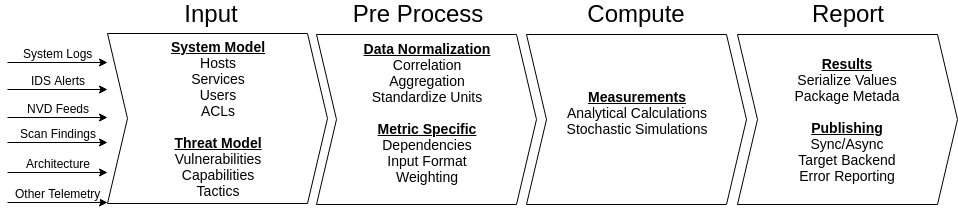
\includegraphics[width=\linewidth]{resource/img/ch_intro/metric_calc_pipeline.png}
\caption{Generalized Metric Evaluation Pipeline}
\label{fig:automation:metric_pipeline}
\end{figure} 

In Figure \ref{fig:automation:metric_pipeline} we present a general four-stage pipeline for security metric processing based on our observations implementing a number of metrics from the literature. This abstraction encourages us to:
\begin{itemize}
\item Decouple the source of system information from the representation of that information. 
\item Decouple the actual calculation of the metric from the input model representation it is typically paired with in its publication. 
\item Decouple the calculation logic and supporting metadata from any assumptions about how that measured value will be used in the future. 
\end{itemize}

In doing so, it becomes possible to identify shared dependencies among metrics, enables a systematic examination of the characteristics and behaviours of each metric across a range of inputs, and supports more reusable and composeable components for a greater variety of deployment scenarios. The remainder of this section provides the considerations and details of each stage.

\subsection{Input Modeling}\label{sec:automation:methodology:inputs}
% \textbf{Input Modeling}

In the \textit{Input} stage of Figure \ref{fig:automation:metric_pipeline}, system details depicted above the inbound arrows on the left are parsed into a model which describes the current environment or environment under test. Model parameters can be populated synthetically or from a live system. Rules comprising the threat model which describes how these components are allowed to interact with each other and with external stimulus can be added here for metrics that require it. The raw inputs to the processing pipeline can vary widely depending on which security metrics are being considered. At a high level, we treat the input stage as a black box for handling information requests from subsequent stages. This affords us the freedom to connect static data for testing and experimentation, and live data for production deployments without altering the contract or interface. In practice input targets can be existing APIs provided by SIEMs, query interfaces to a configuration database, source code repositories, vulnerability information feeds, generated network topologies, etc. At this stage we only assume appropriate adapters exist to make this data available for the subsequent stages.

\subsection{PTaH: Preprocessing and Transformation Handling} \label{sec:automation:methodology:preprocess}
% \textbf{PTaH: Preprocessing and Transformation Handling}

The \textit{Pre Process} stage transforms the current knowledge base into a format suitable for the desired metric calculation. 

% \begin{figure}[ht]
% \centering
% % \includegraphics[width=.5\linewidth]{img/Ptah_archs.png}
% \includegraphics[width=.5\linewidth]{resource/img/ch_benchmarking/secmet_ptah/Ptah_archs.png}
% \label{fig:automation:ptah_arch}
% \end{figure} 

\begin{figure}[ht]
\centering
\includegraphics[width=.5\linewidth]{resource/img/ch_benchmarking/secmet_ptah/Ptah_archs.png}
\caption{Preprocessing and Transformation Handlers (\textbf{PTaH})}
\label{fig:automation:ptah_arch}
\end{figure} 

In metrics that compute aggregates, ratios, or simple statistics from findings and system facts, preprocessing steps may be minimal or bypassed entirely. In more complex metrics, such as those which consider the relationships between components or vulnerabilities, it may be necessary to craft the inputs expected from some composition of system facts along with some composition or chain of metric dependencies. In particular, metrics based on attack graphs and attack nets tend to make assumptions about the input structure which can be managed in this layer. We create these structures, score transitions, apply weights and mappings, and perform any other manipulations of our knowledge base in this layer to adhere to the input assumptions of particular metrics in this layer. 




\subsection{SecMet: A Library of Security Metrics} \label{sec:automation:methodology:compute}
% \textbf{SecMet: A Library of Security Metrics}

The \textit{Compute} stage implements the calculation of the security metric and takes the measurement of the current state. 

% The surveys we covered in Section \ref{sec:background:existing_metrics_taxonomies} describe properties common to all the security metrics they consider, which become evaluation criteria for their review. All security metrics inherit from a parent metric class that defines these common properties and the current system model, along with housekeeping functions and metadata like citations and usage.The security metric does not contain logic to create the inputs it operates on, so we can stack metrics to run in parallel against a single source of facts, or chain them in a processing pipeline to compose more complex analytics. 


% Our architecture for implementing security metrics is straight forward. We declare a \textit{base security metric} type from which all metrics inherit three methods: 
% \begin{itemize}
% \item Check Prerequisites: is invoked either directly by the caller or in the calculate method to ensure all items necessary for the calculation are present.
% \item Calculate: returns the resulting measurement
% \item Get Metadata: returns the environment and ancillary data used during the calculation. 
% \end{itemize}
 

\begin{figure}[H]
\centering
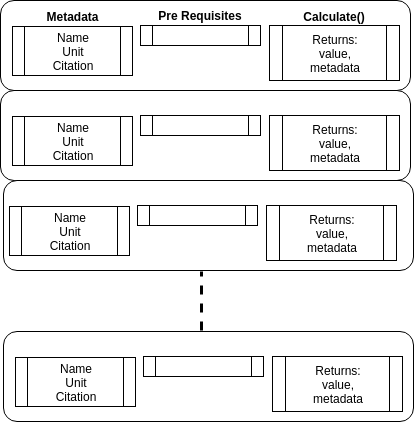
\includegraphics[width=.5\linewidth]{resource/img/ch_benchmarking/secmet_ptah/SecMet_archs.png}
\caption{Security Metric Catalog (\textbf{SecMet})}
\label{fig:automation:metric_arch}
\end{figure} 

As shown in Figure \ref{fig:automation:metric_arch}, this design allows us to implement a library of security metrics with a standard, stateless interface.


% The attack graphs described in the literature vary somewhat in structure among implementations. For example, the AGs presented in \cite{Ou_Appel_2005} include non-exploits along with exploits as nodes with edges representing lateral movements. In \cite{Noel_Jajodia_2014} the non-exploit nodes don't appear to be present in the publication, although the TVA tool isn't publicly available to test this. In \cite{Dacier_1994} and \cite{Ortalo_1999} nodes represent system privileges and edges contain exploits that grant an attacker additional privileges on a set of systems, while in \cite{Phillips_Swiler_1998} edges carry probabilities of exploitation and the nodes represent actual hosts. While the differences are subtle, they are enough to necessitate a general form of attack graph which we present in Figure \ref{fig:automation:ag_uml}. Our representation of an attack graph is a multi-edged directed acyclic graph.     

% % \begin{wrapfigure}[10]{I}{.25\textwidth}
% \begin{figure}[H]
% \centering
% 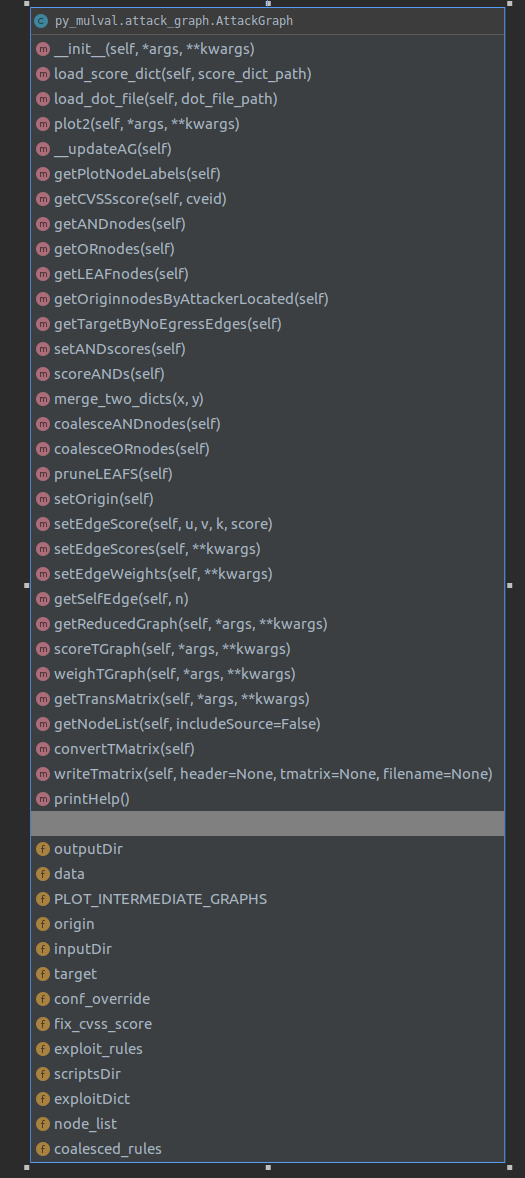
\includegraphics[scale=.45]{resource/img/ch_automation/attack_graph_class_diag.png}
% % \end{wrapfigure}
% \caption{Attack Graph Methods and Properties}
% \label{fig:automation:ag_details_uml}
% \end{figure}

% As shown in Figure \ref{fig:automation:ag_details_uml}, our implementation allows us to load various AG formats from graph description language (.dot) files, from adjacency lists as shown in Tables \ref{tab:eg_verts} and \ref{tab:eg_arcs}, or other formats as specified. Once loaded, we provide programmatic access to manipulate scoring and weighting functions, exploits definitions, and vulnerability scores. This allows for a simple means to test the range of values a metric will generate, the sensitivity of a metric to fluctuations in parameters, and how well a metric performs on different models. It also gives us some insights into how well each AG type actually models threat and defense attributes.




\subsection{Measurement Reporting}\label{sec:automation:methodology:report}
% \textbf{Measurement Reporting}

Finally, the \textit{Reporting} stage handles the response logic needed to return the measured value and associated metadata appropriately. In our experience, most security metrics return a single value, although heuristics are also supported as bucket sizes and value count arrays returned within the accompanying metadata. In these cases we return a value of -1 and a unit of the type to expect in the metadata, eg array or matrix. The metadata['value'] key then points to the resulting complex structure.